\chapter{Key-Value Store Implementation}

Having presented the problem of consensus and the constituent parts of Raft, this paper's implementation of a simple consistent distributed database can now be examined. The source code is freely available as a GitHub repository \cite{stoufexis-raft}.

\section{Key-Value Stores}

The distributed database implemented in this paper is a key-value store. Key-value stores are NoSQL databases that store data as pairings of keys and values. A key is thought to uniquely identify a value; thus, the store behaves like an associative array. Usually, key-value stores do not provide built-in methods for managing the schema of values and do not support complex querying.\\

Key-value stores can support a multitude of use-cases, such as metadata storage, dynamic configuration, caching, and the implementation of high-volume aspects of services, such as shopping-carts \cite{aws-kv-stores,consul-kv-stores}. They are quite useful in distributed setups, as their data-sets can be easily partitioned or replicated and can usually support operations on large data volumes with minimal latency \cite{aws-kv-stores}.\\

\section{Overview of the Implementation} \label{impl-overview}

The implemented database runs as a cluster of servers, along with a reverse proxy, which abstracts the server locations. A REST API is exposed to the user, supporting the retrieval, insertion, and update of values associated with keys. Additionally, a lightweight transaction mechanism is provided for atomically modifying the data set. Finally, each request from clients is expected to contain a unique command identifier, enabling the implementation of linearizable semantics. Linearizable semantics are explained in Subsection \ref{linearizable-semantics}.\\

Raft is used to achieve consistency within the cluster. The set of key-value pairs forms a Raft state machine, with the initial state of an empty set. Each request maps to a Raft command, which is replicated and committed before applying. With each application, the state machine transitions and produces a response that is returned to the client. Thus, consensus is always reached for each modification of the data-set, making it fault-tolerant and consistent across the cluster.\\

Specifically, the following REST endpoints are provided:
\begin{enumerate}
    \item \lstinline|GET /store/{COMMAND_ID}/?keys={KEY_1}&keys={KEY_2}&...|: Retrieves the values currently associated with a set of keys. Along with the values, an identifier called the revision id is returned which can be used with endpoint 3.
    \item \lstinline|PUT /store/{COMMAND_ID}/?{KEY_1}={VALUE_1}&{KEY_2}={VALUE_2}&...|: Inserts the given key-value pairs. If a key already exists it is updated with the given value. A key-value pair can be deleted by providing an empty value for the key.
    \item \lstinline|PUT /store/tx/{COMMAND_ID}/{REVISION_ID}/?{KEY_1}={VALUE_1}&{KEY_2}={VALUE_2}&...|: Behaves identically to the previous endpoint, but only takes effect if a set of reference keys have not been modified since they were previously read. The reference keys are validated through the revision id, which must also be given.
\end{enumerate}

Any client may address a request to any of the servers in the Raft cluster, but the response may be a redirection to another server if the reached server is not the leader.\\

It is worth pointing out that, even though the Raft log is persisted to disk, a snapshot of the latest state of the key-value store is always held in memory. This decreases latency, as the state does not need to be rebuilt from the Raft log on each operation. On the flip-side, it restricts the size of the data-set to the size of the available memory of each machine hosting the Raft servers. Since the main goal of key-value store implementation was simplicity and understandability, this bottleneck was not further optimized. In real-world implementations, part of the data-set may be offloaded to disk.

\subsection{Implementing Transactions} \label{implementing-transactions}

The third listed endpoint can be used to implement transactions via simple optimistic locking \cite{kung1981optimistic} using the following process:
\begin{enumerate}
    \item A client reads any set of keys using the first endpoint, retrieving their value along with a revision id which uniquely identifies their current state. The read keys are used as the reference keys.
    \item Then, the client, knowing the current values of the reference keys, attempts to insert any set of key-value pairs via the third endpoint. The operation is rejected if any reference key has been modified by another client since it was read. This is achieved by requiring the client to provide the revision id that was retrieved on the first step.
    \item If the operation is rejected, the new values of the reference keys are returned along with the new revision id. The client then retries its operation by issuing a new request to the third endpoint. This read-and-insert cycle completes once an insert succeeds, in which case the operations were executed atomically.
\end{enumerate}

Since this transaction mechanism can use any set of keys as the reference and any set of keys as the input, it can be used to implement any atomic read-and-insert type of operation. Note that this general design is used in many atomic data structures, such as in the \lstinline|getAndUpdate| method of \lstinline|AtomicReference| in Java \cite{get-and-update}. Usage examples of this feature will be given in Subsection \ref{transactions-scenario}.\\

It is also worth noting that the transaction is completely durable, even if the Raft leader, or any server, fails after any of the steps, the transaction can be continued by the subsequent leaders.\\

\section{Programming Language and Tools} \label{language-tools}

Before delving into the implementation details of the key-value store, the tools that were used, including programming languages, methodologies, libraries, services, and platforms, are presented.

\subsection{Programming Language}

The Scala programming language is a strongly typed, expressive language that runs on the JVM. It powers some of the world's largest distributed systems, including large financial platforms, streaming platforms such as Netflix \cite{netflix}, Disney Streaming \cite{disney-streaming} and Spotify \cite{spotify}, social media platforms such as Twitter \cite{x-twitter}, gaming platforms such as Lichess \cite{lichess}, big data frameworks such as Spark \cite{spark}, and many others.\\

Due to its pervasiveness and utility in the implementation of distributed systems, it was picked as the go-to language for this thesis.

\subsection{Programming Style}

Scala's expressiveness and type system facilitate a popular programming style, known as pure functional programming. This style, popularized by the Haskell programming language, models programs as pure mathematical structures and operates on them via well-defined and safe operations that possess provable properties.\\

Modeling programs as purely mathematical structures allows the concise expression of complex logic with minimal effort, while speeding up the development process, reducing the occurrences of bugs, and aiding in the long-term maintenance of the code \cite{pure-fp-scala}. This style of programming was used throughout the implementation of the key-value store, as it is invaluable for implementing complex concurrent algorithms.

\subsection{Libraries}

\begin{itemize}
    \item \textbf{cats-effect}: The cats-effect library is the gold standard for concurrency within the Scala ecosystem. It provides a lightweight, reliable asynchronous runtime for Scala, along with abstractions and data structures for writing asynchronous and concurrent programs. It was used throughout the project to achieve high throughput while preserving the reliability of the system.
    \item \textbf{fs2}: Fs2 integrates with cats-effect and provides an additional purely functional data structure, called a Stream. A Stream represents a discrete, lazily produced sequence of values which allows complex transformations using sequential or concurrent operations. The fs2 Stream was used to implement all the core parts of the key-value store. 
    \item \textbf{http4s}: Http4s is a standard solution for implementing http servers and clients using cats-effect and fs2 in Scala. It was used both for implementing the user-facing REST API and for server-to-server communication within the Raft cluster.
    \item \textbf{log4cats}: Log4Cats provides tools for purely functional logging within the cats-effect ecosystem of libraries. As there was a need for traceability, logging had to be introduced in the project and this library was the go-to tool.
    \item \textbf{circe}: Circe is a JSON library for Scala. It enables the abstract representation of a JSON document, as well as conversions between Scala data types and JSON. Circe was necessary as JSON was the format of choice for server-to-client as well as server-to-server communications in the key-value store.
    \item \textbf{scodec}: Scodec enables conversions between Scala data types and byte streams. It was used for generating and parsing revision ids.
    \item \textbf{sqlite}: Sqlite is a fully embedded SQL database engine that is used for persisting and retrieving data from local storage using SQL. It is probably the most used database engine in the world \cite{sqlite-most-used} and was used as the backbone for the persistence layer of the key-value store.
    \item \textbf{doobie}: Doobie is a JDBC client that integrates with cats-effect and fs2. It was used to communicate with the Sqlite database.
\end{itemize}

\subsection{Other Tools}

\begin{itemize}
    \item \textbf{Sbt}: Sbt is the build tool of choice for most Scala projects. It was used for organizing, packaging, building, and testing the code-base.
    \item \textbf{Sbt Native Packager}: A plugin for Sbt which enables packaging Scala applications into various formats. The key-value store uses this plugin to package the application into a Docker image.
    \item \textbf{Scalafmt}: Scalafmt is a code formatter for Scala. It was used for enforcing formatting rules over the code-base to keep it easily readable.
    \item \textbf{Vscode}: Vscode is a code editor that supports most modern programming languages. It was the main tool for authoring the code-base.
    \item \textbf{Metals}: Metals is a language server that integrates well with Vscode and Sbt. It has advanced linting capabilities and it was used for continually enforcing that the code-base can successfully compile, as well as for executing Sbt actions through Vscode, such as building and running the code.
    \item \textbf{Docker}: Docker has become the tool of choice for packaging applications into images and running these images in containers within a managed runtime. The key-value store deploys its servers as a group of Docker containers and it takes advantage of Docker's networking features.
    \item \textbf{Docker Compose}: Docker Compose is used for configuring and deploying Docker containers in a cluster, based on a configuration file. The key-value store comes with a configuration for deploying an experimental cluster for testing.
    \item \textbf{Nginx}: Nginx is a web server, but it is also used as a reverse proxy, a load balancer, a mail proxy, and in other configurations. The key-value store, in its experimental setup, uses Nginx as a reverse proxy, to abstract the details of the cluster from clients.
    \item \textbf{Git}: Git is the modern standard for version control in software projects and was used for that purpose over the entire code-base. 
    \item \textbf{GitHub}: GitHub is a platform for hosting Git repositories, publishing documentation, executing CI/CD pipelines, and many more use cases. It was used for hosting and publishing the code-base.
\end{itemize}

\section{Source Code}

As all the necessary foundation has been laid out, the source code of the key-value store implementation can now be examined in detail.

\subsection{Modules}

The project is spread between two modules, which are built separately by Sbt; \lstinline|raft| and \lstinline|kvstore|.\\

The \lstinline|raft| module contains a generic implementation of the Raft consensus algorithm. Users of this module need to provide implementations for a set of defined interfaces, known as traits in Scala, describing the state machine, persistence layer, server-to-server communication, and server-to-client communication.\\

The \lstinline|kvstore| module depends on the \lstinline|raft| module, implementing the key-value store by providing implementations for all required interfaces. It uses Sqlite for persistence and HTTP for server-to-server and server-to-client communication. The Doobie library is used for interacting with Sqlite, while the http4s library is used to define and run the necessary HTTP server and client. It also includes configuration for running a simple cluster, used for testing.

\subsection{Packages}

The source-code is further organized into packages for each of the modules.\\

The \lstinline|raft| module includes the following packages:
\begin{itemize}
    \item \lstinline|com.stoufexis.raft|: This is the root package, containing all other packages and top-level definitions that are required for users of the module.
    \item \lstinline|com.stoufexis.raft.model|: Contains definitions of core data types that are used throughout the implementation.
    \item \lstinline|com.stoufexis.raft.persist|: Defines the two traits that users of the module must implement to enable persistence.
    \item \lstinline|com.stoufexis.raft.rpc|: Contains definitions of data types and functions used for server-to-server and server-to-client communications. Some parts of the implementation are missing, allowing users of the module to plug in any underlying technology.
    \item \lstinline|com.stoufexis.raft.statemachine|: Contains the generic Raft implementation and all its core functions and data types. The definition of the state machine to be replicated and its input and output types are not hard-coded, allowing the user to provide any implementation.
    \item \lstinline|com.stoufexis.raft.typeclass|: Contains definitions of type classes \cite{wadler1989make} used in some generic functions.
\end{itemize}

The \lstinline|kvstore| module includes the following packages:
\begin{itemize}
    \item \lstinline|com.stoufexis.raft.kvstore|: This is the root package, containing all other packages and top-level definitions, including the entry-point for running the key-value store application.
    \item \lstinline|com.stoufexis.raft.kvstore.persist|: Uses Sqlite and Doobie to provide implementations for the traits defined in \lstinline|com.stoufexis.raft.persist|.
    \item \lstinline|com.stoufexis.raft.kvstore.rpc|: Uses http4s to plug in an HTTP-based implementation for the missing parts of \lstinline|com.stoufexis.raft.rpc|.
    \item \lstinline|com.stoufexis.raft.kvstore.statemachine|: Provides the definition of the state machine, implementing the core logic of the key-value store, along with its input and output types. The state machine definition is provided to the \lstinline|raft| module, which replicates it across the cluster.
\end{itemize}

\subsection{Data Types and Functions}

Next, a brief description of the defined functions and data types is provided, per package. Parts of the source code deemed entirely self-explanatory or non-essential for the reader's understanding are left out. For a greater level of detail, the reader is encouraged to also inspect the source code in the GitHub repository \cite{stoufexis-raft}.

\subsubsection{Notes on Notation}

In the following lists, a name containing a period denotes one of the following:
\begin{itemize}
    \item A member of a class, trait, or object. The right side is the name of the member while the left side is the class, trait, or object.
    \item An extension function. The right side is the name of the function, while the left side is the type for which the extension function is defined.
\end{itemize}

Additionally, note the following:
\begin{itemize}
    \item Function parameters, type parameters, and return types are not shown, but may be mentioned when required.
    \item Unless specified otherwise, Stream refers to the Stream data type provided by fs2.
\end{itemize}

\subsubsection{\lstinline|com.stoufexis.raft|}

\begin{itemize}
    \item \lstinline|ExternalNode|: Trait representing a handle to a Raft server within the cluster other than the current one. An instance of this trait for every external server is given by users of the package, allowing them to use any technology for sending commands from one Raft server to another.
    \item \lstinline|ExternalNode.id|: Unique identifier of the external Raft server.
    \item \lstinline|ExternalNode.appendEntries|: Sends an \lstinline|AppendEntries| command to the external Raft server. The response should be returned to the Raft instance running on this server. This implements the sending side of the AppendEntries RPC, described in detail in Chapter 3 of the Raft paper \cite{raft}.
    \item \lstinline|ExternalNode.requestVote|: Sends a \lstinline|RequestVote| command to the external Raft server. The response should be returned to the Raft instance running on this server. This implements the sending side of the RequestVote RPC, described in detail in Chapter 3 of the Raft paper \cite{raft}.
    \item \lstinline|RaftNode|: Trait representing a handle to the Raft process running on the current server. An instance of this trait is given to users of the Raft package, allowing them to use any technology for receiving commands from clients or from other servers.
    \item \lstinline|RaftNode.appendEntries|: Provides an \lstinline|AppendEntries| command, sent by an external Raft server, to the Raft process running on this server. A response is produced which is expected to be routed back to the sender-server. This implements the receiving side of the AppendEntries RPC, described in detail in Chapter 3 of the Raft paper \cite{raft}.
    \item \lstinline|RaftNode.requestVote|: Provides a \lstinline|RequestVote| command, sent by an external Raft server, to the Raft process running on this server. A response is produced which is expected to be routed back to the sender-server. This implements the receiving side of the RequestVote RPC, described in detail in Chapter 3 of the Raft paper \cite{raft}.
    \item \lstinline|RaftNode.clientRequest|: Provides a command from a client to the Raft instance running on this server. If the current server is the leader, it attempts to commit the command by replicating it to a majority of servers. Once committed, the state machine is advanced and a response is returned containing the result of the command, which should be routed back to the sender-client. If the current server is not the leader, the response is a redirection to the leader.
    \item \lstinline|RaftNode.Builder|: A data type, implementing the builder pattern, which is used for configuring the Raft process.
    \item \lstinline|RaftNode.builder|: Creates an object of type \lstinline|Builder|, providing default values and allowing for further configuration. It requires a unique identifier of the current Raft server, the definition of the state machine to be replicated, and instances of the traits implementing the persistence layer.
    \item \lstinline|RaftNode.Builder.withExternals|: Configures the Raft process of the current server by providing handles to the rest of the servers within the cluster.
    \item \lstinline|RaftNode.Builder.withHeartbeatEvery|: Configures the heartbeat interval used by the Raft process.
    \item \lstinline|RaftNode.Builder.withElectionTimeout|: Configures the election timeout range used by the Raft process.
    \item \lstinline|RaftNode.Builder.withAppenderBatchSize|: Configures the batch size used by the leader when attempting to replicate multiple log entries at once.
    \item \lstinline|RaftNode.Builder.build|: Uses the configuration parameters given to the \lstinline|Builder| to create a \lstinline|RaftNode| instance.
\end{itemize}

\subsubsection{\lstinline|com.stoufexis.raft.model|}

\begin{itemize}
    \item \lstinline|Command|: The pairing of a user-defined command type with a command id.
    \item \lstinline|CommandId|: The unique identifier of a command.
    \item \lstinline|Index|: The sequence number of entries in the replicated log.
    \item \lstinline|Index.init|: The index number of the first entry in the replicated log.
    \item \lstinline|Index.uninitiated|: The index number preceding the \lstinline|init| index.
    \item \lstinline|NodeId|: The unique identifier of a Raft server within the cluster.
    \item \lstinline|Role|: An enumeration representing the state of the current server, either Follower, Candidate, or Leader.
    \item \lstinline|Role.init|: The \lstinline|Role| with which each server starts up.
    \item \lstinline|Term|: The Raft term.
    \item \lstinline|Term.init|: The initial Raft term.
    \item \lstinline|Term.uninitiated|: The term preceding the \lstinline|init| term.
\end{itemize}

\subsubsection{\lstinline|com.stoufexis.raft.persist|}

\begin{itemize}
    \item \lstinline|Log|: Trait enabling the persistence of the Raft log to disk. Users of the \lstinline|raft| package are expected to provide concrete implementations of this trait to the Raft process, which allows them to use any persistence technology.
    \item \lstinline|Log.append|: Appends and persists a non-empty sequence of commands to the Raft log, returning the index of the last entry.
    \item \lstinline|Log.commandIdExists|: Checks whether the log contains a command, given a command id.
    \item \lstinline|Log.matches|: Checks whether there exists an entry in the log with the given index and term. If true, all log entries up to the given index are guaranteed to be identical. This is due to the Log Matching property of Raft as described in Section \ref{raft-properties}.
    \item \lstinline|Log.deleteAfter|: Deletes all log entries after the given index.
    \item \lstinline|Log.range|: Returns all log entries between two indexes.
    \item \lstinline|Log.rangeStream|: Returns all log entries between two indexes as an fs2 Stream.
    \item \lstinline|Log.lastTermIndex|: Returns the term and index of the last entry in the log.
    \item \lstinline|Log.term|: Returns the term of the entry with the given index. If the entry does not exist, an error should be raised, but this function is guaranteed by the Raft implementation to only be called with valid indexes.
    \item \lstinline|PersistedState|: Trait enabling the persistence of data, additional to the Raft log, to disk. The only additional data required by Raft is the candidate for which a server voted during each term's leader election. This ensures that a server can never vote twice in a single term.
    \item \lstinline|PersistedState.persist|: Persists the vote for the given term. If no vote has been made, a \lstinline|None| should be given.
    \item \lstinline|PersistedState.readLatest|: Returns the persisted vote for the latest term.
\end{itemize}

\subsubsection{\lstinline|com.stoufexis.raft.rpc|}

\begin{itemize}
    \item \lstinline|AppendEntries|: The message instructing a follower to append a sequence of entries to its internal log.
    \item \lstinline|AppendResponse|: The response sent by a server after it receives an \lstinline|AppendEntries| message from a leader. It signals success when the entries were successfully appended. Additionally, it may signal failure when the leader's log is not consistent with the follower's or it has a stale term.
    \item \lstinline|RequestVote|: The message soliciting a vote from a server.
    \item \lstinline|VoteResponse|: The response sent by a server after it receives a \lstinline|RequestVote| message from a candidate. It signals whether the vote is granted or rejected. Additionally, it may signal failure when the candidate's term is stale.
    \item \lstinline|ClientResponse|: The response returned to a client by a server after attempting to apply a command. It can signal success by returning the current state along with any output produced by the state machine. Additionally, if the server receiving the command is not the leader, it will redirect to the leader, or inform the client that the leader is not known. Finally, it can inform the client that the command was skipped, which happens when its id was not unique. The conditions for skipping a command are further explained in Subsection \ref{linearizable-semantics}.
    \item \lstinline|ClientResponse.knownLeader|: Constructs a \lstinline|ClientResponse| containing the current leader or informing the client that there is no known leader.
    \item \lstinline|IncomingAppend|: Message used to implement the receiving side of an AppendEntries RPC. It pairs an \lstinline|AppendEntries| message along with a handle for providing an \lstinline|AppendResponse|.
    \item \lstinline|IncomingClientRequest|: Message used to implement the fulfillment of \lstinline|ClientRequest|s. It pairs a \lstinline|Command| along with a handle for providing a \lstinline|ClientResponse|.
    \item \lstinline|IncomingVote|: Message used to implement the receiving side of a RequestVote RPC. It pairs a \lstinline|RequestVote| message along with a handle for providing a \lstinline|VoteResponse|.
    \item \lstinline|InputVotes|: Trait used to implement the receiving side of RequestVote RPCs.
    \item \lstinline|InputVotes.incomingVotes|: Provides a Stream of all \lstinline|IncomingVote|s.
    \item \lstinline|InputAppends|: Trait used to implement the receiving side of AppendEntries RPCs.
    \item \lstinline|InputAppends.incomingAppends|: Provides a Stream of all \lstinline|IncomingAppend|s.
    \item \lstinline|InputClients|: Trait used to implement the fulfillment of \lstinline|ClientRequest|s.
    \item \lstinline|InputClients.incomingClientRequests|: Provides a Stream of all \lstinline|IncomingClientRequest|s.
    \item \lstinline|InputSource|: Extends from the \lstinline|InputVotes|, \lstinline|InputAppends|, and \lstinline|InputClients| traits, allowing receiving all three message types.
    \item \lstinline|InputSink|: Trait used to implement the methods of \lstinline|RaftNode|. It receives requests from external servers and clients, routes them to the Raft process, and returns the response for each request back to them.
    \item \lstinline|InputSink.requestVote|: Used to implement the \lstinline|requestVote| method of \lstinline|RaftNode|.
    \item \lstinline|InputSink.appendEntries|: Used to implement the \lstinline|appendEntries| method of \lstinline|RaftNode|.
    \item \lstinline|InputSink.clientRequest|: Used to implement the \lstinline|clientRequest| method of \lstinline|RaftNode|.
    \item \lstinline|Inputs|: Extends from \lstinline|InputSource| and \lstinline|InputSink|, packaging them in one trait for easier usage.
    \item \lstinline|Inputs.apply|: Creates an instance of the \lstinline|Inputs| trait by implementing the receiving and sending side of each message type using 
    \lstinline|RequestQueue|s. Each of the sending methods enqueues an element while each of the receiving methods consumes elements from the queues as a Stream.
    \item \lstinline|RequestQueue|: A special implementation of a purely-functional, concurrent, bounded queue, holding requests. Enqueued elements are ordered in normal FIFO fashion, but they are not removed from the queue immediately when dequeued. Instead, a request is "committed" and removed when the consumer of the queue provides a response for it. This maintains elements in the queue during state transitions, without losing dequeued requests and without blocking the transition until they are processed. If an element is dequeued but its processing is interrupted because of a state transition, e.g. from Leader to Follower, it remains in the queue and is picked up by the Raft process in the next state, as it was not committed.
    \item \lstinline|RequestQueue.consume|: Consumes from the queue by receiving a Stream of uncommitted elements, along with a handle for committing them.
    \item \lstinline|RequestQueue.offer|: Offers an element to the queue and awaits for it to be committed, returning the response. If the queue has reached its bound, the offer will wait until there is room.
    \item \lstinline|RequestQueue.tryOffer|: Offers an element to the queue and awaits for it to be committed, returning the response. If the queue has reached its bound, the offer immediately returns a value of \lstinline|None| instead of waiting.
    \item \lstinline|RequestQueue.apply|: Creates a \lstinline|RequestQueue| with the given bound.
    \item \lstinline|RequestQueue.Unprocessed|: Utility class used to implement the core internal operations of the \lstinline|RequestQueue|.
    \item \lstinline|RequestQueue.Unprocessed.tryOffer|: Internal method used to implement \lstinline|RequestQueue.tryOffer|.
    \item \lstinline|RequestQueue.Unprocessed.offer|: Internal method used to implement \lstinline|RequestQueue.offer|.
    \item \lstinline|RequestQueue.Unprocessed.drop|: Drops an element from the queue after it is committed. It's an internal method used to implement \lstinline|RequestQueue.offer| and \lstinline|RequestQueue.tryOffer|.
    \item \lstinline|RequestQueue.Unprocessed.read|: Internal method used to implement \lstinline|RequestQueue.consume|.
    \item \lstinline|RequestQueue.Unprocessed.apply|: Creates an instance of the \lstinline|Unprocessed| class by initializing its internal state. It allows for the state's concurrent access by wrapping it in a cats-effect \lstinline|Ref|.
    \item \lstinline|RequestQueue.State|: Used to hold the internal state of the \lstinline|RequestQueue|. It contains the index of the last element of the queue, a \lstinline|Map| containing all the currently uncommitted elements, and a Scala \lstinline|Queue| holding handles to fibers that are waiting to enqueue an element.
    \item \lstinline|RequestQueue.State.elemsBetween|: Helper function that returns all uncommitted elements within a range of indexes.
    \item \lstinline|RequestQueue.State.empty|: Constructs an object of \lstinline|RequestQueue.State| with an index of 0, an empty \lstinline|Map| of elements, and an empty Scala \lstinline|Queue| of waiting fibers.
\end{itemize}

\subsubsection{\lstinline|com.stoufexis.raft.statemachine|}

\begin{itemize}
    \item \lstinline|AppenderCfg|: Case class configuring the heartbeat interval and the batch size used when appending entries.
    \item \lstinline|Automaton|: Case class containing the definition of the user-provided state machine.
    \item \lstinline|Automaton.apply|: Transitions the state machine by providing the current state and an input command from a client. The result of the transition is the new state, along with an output message that should be returned to the client.
    \item \lstinline|Behaviors|: Holds a list of processes that are to be run concurrently, implementing the various components of each of the three server states. Each process is modeled as Stream, which runs indefinitely, but may terminate by producing a single value. The produced value is of type \lstinline|NodeInfo| and it triggers the transition of the server to a new state.
    \item \lstinline|Behaviors.raceFirst|: Runs all the processes concurrently, waiting for any of them to terminate and produce a value of type \lstinline|NodeInfo|. When a value is produced, all other process are interrupted and the value is returned.
    \item \lstinline|Behaviors.++|: Appends a sequence of processes to the \lstinline|Behaviors| object.
    \item \lstinline|Behaviors.apply|: Creates a Behaviors object with an initial list of processes.
    \item \lstinline|BufferredPublisher|: Trait that wraps an fs2 Topic object and allows for cleanly interrupting its publish methods via a shutdown procedure.
    \item \lstinline|BufferredPublisher.publish|: Publishes a message to the topic, but allows for interruption during the shutdown procedure. Returns true if the message was published successfully and false otherwise
    \item \lstinline|BufferredPublisher.publishOrThrow|: Same as publish, but raises an error if not successful.
    \item \lstinline|BufferredTopic|: Trait extending from \lstinline|BufferredPublisher| that adds a method for registering subscribers to the topic.
    \item \lstinline|BufferredTopic.newSubscriber|: Creates a subscription to the topic that is interrupted during the shutdown procedure. The subscription is modeled as a handle to a Stream of the topic's messages.
    \item \lstinline|BufferredTopic.apply|: Creates an instance of the \lstinline|BufferredTopic| trait. The instance is wrapped in a cats-effect Resource, which ensures that the shutdown procedure is ran after use. The shutdown procedure interrupts all publishers and all subscribers.
    \item \lstinline|Leader|: An object defining all processes that need to be run concurrently when the server is in the leader state.
    \item \lstinline|Leader.apply|: Returns all the leader processes as a \lstinline|Behaviors| object. It creates two instances of \lstinline|BufferredTopic|, which are used for message passing between the processes. One of the topics contains the indexes of new entries in the log. A new index is published to the topic after new entries are written to the log. The second topic contains the match index for each follower servers. An update is published every time the leader successfully appends entries to a follower. Match indexes are explained further in the description of \lstinline|commitIdxFromMatch|.
    \item \lstinline|Leader.votes|: The process responding to vote requests from candidates. Vote requests for the current term are rejected, since the current server is a leader, meaning it has voted for itself. If a request for a newer term is received, the process produces a value signaling the server to fallback to a follower state with an unknown leader. Requests with a stale term are rejected.
    \item \lstinline|Leader.appends|: The process responding to append requests. If a request for a newer term is received, the process produces a value signaling the current server to transition to a follower state, since another server is the leader. Requests with a stale term are rejected.
    \item \lstinline|Leader.commitIdxFromMatch|: Helper function that calculates the commit index from the match indexes of followers. The match index is a position of a follower's log, which marks the latest entry where the follower's log matches completely with the leader's. Calculating it becomes simpler due to the Log Matching property of Raft; the match index is simply the largest index containing a log entry that matches in its index and in its term with an entry from the leader's log. The commit index is calculated as the largest index that is lesser than or equal to the majority of match indexes. Practically, the commit index marks the latest log entry that is present on the majority of the servers' internal logs \cite{raft}.
    \item \lstinline|Leader.stateMachine|: The process accepting commands from clients. Every command is first appended to the internal log. Then, the index of the new command is pushed to one of the topics, instructing the \lstinline|appender| process to replicate it to all followers. The process also listens to updates of match indexes from the other topic and calculates the new commit index after every update using \lstinline|commitIdxFromMatch|. Every time the commit index is incremented, the command matching that index is considered committed and is applied to the state machine, which returns the new state and an output. The output and the new state are sent as a response to the client who sent the command. Many clients may be concurrently waiting for their command to be applied, with a bound on their number enforced by the \lstinline|RequestQueue| backing the process.
    \item \lstinline|Leader.partitionChecker|: The process constantly checking whether a network partition has happened that isolated the current server from the majority of the cluster. If the \lstinline|appender| process does not produce updates in the match index topic from the majority of the cluster for a time period exceeding the election timeout, a partition is detected. When a partition is detected, the server falls back to a follower state. This process is not mandatory for Raft's safety, as a partitioned leader can never modify the replicated log. However, it is useful for a partitioned leader to quickly become a follower even before the partition is solved, so that any clients can stop attempting to address their commands to it.
    \item \lstinline|Leader.appender|: The process tasked with replicating log entries to followers. Each time the \lstinline|stateMachine| process appends an entry to the log, it also publishes the index of the entry to a topic. This process reads from the topic and attempts to replicate the command matching the index to all followers. Each time a command is successfully replicated to a follower, an update is produced to the match index topic. Additionally, if there are no new commands for the duration of a heartbeat interval, the process sends heartbeat requests to each follower. Heartbeat requests are identical to normal replication requests, but contain no entries to be replicated. A successful heartbeat request results in the process re-sending the current match index of the follower to the topic, signaling that it was reachable, but no new entries were replicated.
    \item \lstinline|Candidate|: An object defining all processes that need to be run concurrently when the server is in the candidate state.
    \item \lstinline|Candidate.apply|: Returns all the candidate processes as a \lstinline|Behaviors| object.
    \item \lstinline|Candidate.appends|: The process responding to append requests. If a valid request is received, the process produces a value signaling the current server to transition to a follower state, since another server has become the leader. Requests with a stale term are rejected.
    \item \lstinline|Candidate.inVotes|: The process responding to vote requests from other candidates. Vote requests for the current term are rejected, since the current server is a candidate, meaning it has voted for itself. If a request for a newer term is received, the process produces a value signaling the server to fallback to a follower state with an unknown leader. Requests with a stale term are rejected.
    \item \lstinline|Candidate.solicitVotes|: The process sending vote requests to the rest of the cluster, attempting to win the election. If a majority votes is gathered, the process produces a value signaling the server to transition to a leader state. Note that the candidate always implicitly votes for itself.
    \item \lstinline|Follower|: An object defining all processes that need to be run concurrently when the server is in the follower state.
    \item \lstinline|Follower.apply|: Returns all the follower processes as a \lstinline|Behaviors| object.
    \item \lstinline|Follower.isUpToDate|: Helper function checking if a candidate's log is at least as up-to-date as the current server's log. This implements the additional election rule described in Subsection \ref{leader-election-fault-tolerance}.
    \item \lstinline|Follower.votes|: The process responding to vote requests from candidates. If the follower has already voted for this term, all requests for the term are rejected, otherwise, the first one wins. A request containing a new term causes the current vote, if one exists, to be dropped. Requests with a stale term are rejected.
    \item \lstinline|Follower.appends|: The process responding to append requests. Each time the leader sends an append request, it is validated and appended to the follower's internal log. During validation, the \lstinline|prevLogTerm| and \lstinline|prevLogIndex| attributes are extracted from the request. These two match the index and term of the entry in the leaders log right before the entries in the request. The follower looks up if there is any entry in its own log matching these two. If successful, every entry up to and including the entry matching the \lstinline|prevLogIndex| are identical between the leader and the follower, due to the Log Matching property. The validation then succeeds and the follower adds the entries to its log, right after the position indicated by \lstinline|prevLogIndex|, replacing any conflicting entries. If the validation fails, the follower rejects the request, informing the leader that the logs up to the provided index are inconsistent. The leader then keeps retrying by sending entries, each time starting at an older index, until a consistent point is found. Requests with a stale term are rejected.
    \item \lstinline|Cluster|: A case class containing the unique id of the current server, as well as handles to all other servers in the cluster.
    \item \lstinline|Cluster.allNodes|: The identifiers of all servers in the cluster.
    \item \lstinline|Cluster.otherNodeIds|: The identifiers of all servers in the cluster, excluding the current one.
    \item \lstinline|Cluster.otherNodesSize|: The number of servers in the cluster, excluding the current one.
    \item \lstinline|Cluster.majorityCnt|: How many servers constitute a majority in the current cluster.
    \item \lstinline|Cluster.isMajority|: Function that checks if the provided set of server ids form a majority. The function excludes any server ids that are unknown and then counts the remaining ones.
    \item \lstinline|Deps|: A case class aggregating common parameters of functions within the package.
    \item \lstinline|ElectionTimeout|: A utility for retrieving an election timeout interval.
    \item \lstinline|ElectionTimeout.nextElectionTimeout|: Picks a random election timeout interval from a range.
    \item \lstinline|ElectionTimeout.fromRange|: Creates an \lstinline|ElectionTimeout| object by providing a range of time intervals.
    \item \lstinline|NamedLogger|: Utility for creating a logger with a readable name.
    \item \lstinline|NamedLogger.fromState|: Creates a logger with a name derived from the server's current state.
    \item \lstinline|NodeInfo|: Case class containing core information about a server's state; the current \lstinline|Role|, \lstinline|Term|, and the leader of the cluster, if it is known.
    \item \lstinline|NodeInfo.toFollower|: Overloaded method returning a new \lstinline|NodeInfo| based on the current one, switching the role to follower with a known leader. A new term can optionally be provided.
    \item \lstinline|NodeInfo.toFollowerUnknownLeader|: Overloaded method returning a new \lstinline|NodeInfo| based on the current one, switching the role to follower with an unknown leader. A new term can optionally be provided.
    \item \lstinline|NodeInfo.toVotedFollower|: Method returning a new \lstinline|NodeInfo| based on the current one, switching the role to follower with an unknown leader but with a registered vote for the current term.
    \item \lstinline|NodeInfo.toCandidateNextTerm|: Method returning a new \lstinline|NodeInfo| based on the current one, switching the role to candidate for the next term.
    \item \lstinline|NodeInfo.toLeader|: Method returning a new \lstinline|NodeInfo| based on the current one, switching the role to leader for the current term.
    \item \lstinline|NodeInfo.isNew|: Method checking if the provided term is newer than the current one.
    \item \lstinline|NodeInfo.isNotNew|: Negation of \lstinline|isNew|.
    \item \lstinline|NodeInfo.isExpired|: Method checking if the provided term is stale.
    \item \lstinline|NodeInfo.isCurrent|: Method checking if the provided term is the current term.
    \item \lstinline|NodeInfo.isLeader|: Method checking if the provided id corresponds to the known leader.
    \item \lstinline|NodeInfo.isCurrentLeader|: Method checking if the provided id corresponds to the known leader and the provided term is the current one.
    \item \lstinline|NodeInfo.isVotee|: Method checking if the provided id corresponds to the candidate that has the current server's vote for the current term.
    \item \lstinline|NodeInfo.isCurrentVotee|: Method checking if the provided id corresponds to the candidate that has this server's vote for the current term and that the provided term is the current one.
    \item \lstinline|NodeInfo.hasVoted|: Method checking if the current server is acting as a follower and has voted for a server.
    \item \lstinline|NodeInfo.votedFor|: Method returning the candidate that this server has voted for in the current term, if it is acting as a follower. If the current server is not a follower or it has not voted, a \lstinline|None| value is returned.
    \item \lstinline|StateMachine|: Entry point for running the internal Raft process.
    \item \lstinline|StateMachine.runLoop|: Runs the Raft process. First, it reads the persisted vote from the server's local storage, if there is one. This ensures that no votes are lost if this server had failed before and is now restarting. Then, it assumes the role of follower and runs the follower's processes by calling the \lstinline|raceFirst| function of the follower's \lstinline|Behaviors| object. It then awaits the termination of \lstinline|raceFirst|, which produces a value, informing the run loop of the next state it should transition to. The run loop constructs the \lstinline|Behaviors| object corresponding to the new state, and runs \lstinline|raceFirst| again. The server's vote is persisted between each transition, if one was made for the term. The loop runs indefinitely. Note that the function is non-tail recursive, which is made safe by cats-effect, as it provides stack-safe monadic recursion \cite{freeman2015stack}.
    \item \lstinline|WaitingClient|: Provides operations on a queue of clients waiting for their commands to be committed and a response to be returned. These operations are used to implement \lstinline|Leader.stateMachine|.
    \item \lstinline|WaitingClient.enqueue|: Adds a waiting client to the queue. A waiting client is modeled as the index of the command that the client sent, as well as a handle to provide a response.
    \item \lstinline|WaitingClient.fulfill|: Provided the current commit index and the current state of the state machine, it applies all commands from clients up to the commit index and returns a response to each of them. It returns the resulting state of the state machine along with any remaining clients that did not get a response, as their commands' indexes were greater than the commit index.
    \item \lstinline|ResettableTimeout|: Data type used to implement \lstinline|resettableTimeoutAccumulate|, modeling the three types of supported signals.
    \item \lstinline|ResettableTimeout.outputPure|: Creates an instance of \lstinline|ResettableTimeout| signaling the emission of a value with no side effects.
    \item \lstinline|Stream.resettableTimeoutAccumulate|: A function continually pulling from a Stream and applying a stateful transformation that can be interrupted after a timeout. The function returns a new Stream that produces only a single value, or gets interrupted after a timeout. The caller of this function has to provide an initial state, a timeout duration, an effect to be executed upon a timeout, and a function modeling the stateful transformation. The output of the function is of type \lstinline|ResettableTimeout|, allowing it to signal the reset of the timeout, the skipping of a value, or the output of a value.
    \item \lstinline|Stream.increasing|: Transforms a Stream of numeric elements by only keeping elements that were greater than any preceding ones.
    \item \lstinline|Stream.dropping|: Applies back-pressure to a Stream by internally buffering a set amount of elements. If new elements arrive when the buffer is full, it makes space by dropping old elements. A new Stream is returned, which reads from the internal buffer, emptying it. This ensures that a slow consumer of a Stream will not have to catch up by reading a large amount of enqueued elements. Rather, it will only have to read up to a set amount.
    \item \lstinline|Stream.repeatLast|: Returns a Stream that produces elements pulled from the provided stream, but repeats the last produced element after a period of inactivity.
    \item \lstinline|Stream.mergeEither|: Concurrently merges two Streams by returning a new Stream. The new Stream produces values of the first Stream wrapped in \lstinline|Either.Left| and values from the second Stream wrapped in \lstinline|Either.Right|.
    \item \lstinline|raceFirst|: Overloaded function concurrently pulling from a list of Streams. When one of the Streams produces a value, all streams are interrupted and the value is returned.
    \item \lstinline|raceFirstOrError|: Same as \lstinline|raceFirst| but raises an error if all Streams terminate without producing a value.
    \item \lstinline|AppendEntries.termExpired|: Responds to an \lstinline|AppendEntries| request, rejecting it and informing the requester that its term is stale.
    \item \lstinline|AppendEntries.duplicateLeaders|: Responds to an \lstinline|AppendEntries| request, informing the requester that duplicate leaders have been detected for a term. Then, it raises an error. Duplicate leaders for a term can never be created by Raft, so this is an unrecoverable error, indicating a bug in the implementation.
    \item \lstinline|AppendEntries.accepted|: Responds to an \lstinline|AppendEntries| request, informing that it has been accepted.
    \item \lstinline|AppendEntries.inconsistent|: Responds to an \lstinline|AppendEntries| request, rejecting it and informing the requester that the its log is inconsistent with the current server's.
    \item \lstinline|RequestVote.termExpired|: Responds to a \lstinline|RequestVote| request, rejecting it and informing the requester that its term is stale.
    \item \lstinline|RequestVote.reject|: Responds to a \lstinline|RequestVote| request, denying to vote for the requester.
    \item \lstinline|RequestVote.grant|: Responds to a \lstinline|RequestVote| request, granting the vote to the requester.
    \item \lstinline|Stream.respondWithLeader|: Responds to a command from a client, informing that the current server is not the leader and returning the actual leader's id, if it is known.
\end{itemize}

\subsubsection{\lstinline|com.stoufexis.raft.typeclass|}

\begin{itemize}
    \item \lstinline|Empty|: Type class providing an empty value associated with a type.
    \item \lstinline|Empty.empty|: The empty value associated with a type.
    \item \lstinline|Empty.const|: Creates an instance of \lstinline|Empty| that always returns the given value when \lstinline|empty| is called.
    \item \lstinline|Empty.derived|: Automatically creates an instance of \lstinline|Empty| for case classes containing elements that already have \lstinline|Empty| instances defined.
    \item \lstinline|Empty.getAll|: Gathers the \lstinline|Empty| instances of all types contained in a case class and returns them as a \lstinline|Tuple|.
    \item \lstinline|IntLike|: Type class providing numeric operations for any type that resembles an integer.
    \item \lstinline|IntLike.add|: Enables adding a value of type \lstinline|Int| to values of a type implementing \lstinline|IntLike|.
    \item \lstinline|IntLike.toLong|: Enables converting values of a type implementing \lstinline|IntLike| to \lstinline|Long|.
\end{itemize}

\subsubsection{\lstinline|com.stoufexis.raft.kvstore|}

\begin{itemize}
    \item \lstinline|KvStoreConfig|: Case class aggregating all configuration parameters for the key-value store implementation.
    \item \lstinline|KvStoreConfig.loadFromEnv|: Creates an instance of \lstinline|KvStoreConfig| by loading all configuration parameters from environment variables.
    \item \lstinline|Main|: Contains the entry-point for the key-value store application.
    \item \lstinline|Main.raftNode|: Starts up the Raft process and returns a handle of type \lstinline|RaftNode|.
    \item \lstinline|Main.server|: Runs the HTTP server handling all server-to-server and server-to-client communications.
    \item \lstinline|Main.run|: The entry-point for the application. Starts up the Raft process and the HTTP server.
\end{itemize}

\subsubsection{\lstinline|com.stoufexis.raft.kvstore.persist|}

\begin{itemize}
    \item \lstinline|SqlitePersistence|: Contains implementations for the two traits comprising the persistence layer of Raft: \lstinline|Log| and \lstinline|PersistedState|.
    \item \lstinline|SqlitePersistence.apply|: Creates an instance for \lstinline|Log| and \lstinline|PersistedState| by delegating to an embedded Sqlite database. The database schema is detailed in Subsection \ref{sqlite-schema}.
\end{itemize}

\subsubsection{\lstinline|com.stoufexis.raft.kvstore.rpc|}

\begin{itemize}
    \item \lstinline|Routes|: Contains the definitions of HTTP endpoints used for server-to-server and server-to-client communications.
    \item \lstinline|Routes.apply|: Creates and returns an object describing all HTTP endpoints. The endpoints used by clients are described in the introduction of Section \ref{impl-overview}, while the endpoints used by servers are described in Subsection \ref{rpc-endpoints}.
    \item \lstinline|RpcClient|: Contains the implementation of the \lstinline|ExternalNode| trait for the key-value store.
    \item \lstinline|RpcClient.apply|: Uses an HTTP client to implement \lstinline|ExternalNode|. Each request is retried indefinitely in cases of failure; requests to a server in the cluster that has become non-operational will be re-sent until it becomes operational again and replies, or until the retry loop is interrupted externally.
\end{itemize}

\subsubsection{\lstinline|com.stoufexis.raft.kvstore.statemachine|}

\begin{itemize}
    \item \lstinline|KvCommand|: Data type modeling the three commands supported by the key-value store, described in detail in the introduction of Section \ref{impl-overview}. A client can read, insert, update, or delete the values of a set of keys in a standalone operation or paired atomically with a read.
    \item \lstinline|KvResponse|: Data type modeling the responses produced by the key-value store state machine. Both possible responses signal success, but one carries values associated with keys and a \lstinline|RevisionId|, while the other one has no payload.
    \item \lstinline|KvState|: Data type modeling the state of the key-value store state machine. It keeps track of all key-value pairs in the store along with a revision, indicating when each was last modified. Additionally, it manages the global revision, which is modeled as a \lstinline|Long|. Note that the revision is incremented after each update to the store, and there currently is no mechanism to handle overflows. This means that after 9,223,372,036,854,775,807 modifications, the store will assume undefined behavior. Assuming an exaggerated rate of 100,000 operations a second, the revision will overflow after around 300,000 years of operation, meaning there is no immediate need for concern. Of course, the implementation can also be modified to handle overflows gracefully.
    \item \lstinline|KvState.setAll|: Returns a new \lstinline|KvState| object that modifies the current state by applying a \lstinline|Map| containing key-value pairs. The \lstinline|Map| may contain values for new keys, new values for existing keys, or indicate the deletion of a key, by pairing the key with a \lstinline|None| value. The new state contains an incremented global revision and any keys modified or added are assigned this id.
    \item \lstinline|KvState.revisionMatches|: Checks if the given \lstinline|RevisionId| matches with the current state. If there is a match, then no modifications have been made since a previous read. This is the step confirming that a modification is being made atomically with a read.
    \item \lstinline|KvState.getAll|: Provided a set of keys, returns all the matching key-value pairs along with their revisions.
    \item \lstinline|KvState.valuesForKeys|: Provided a set of keys, calls \lstinline|getAll| and creates an instance of \lstinline|KvResponse| containing the returned key-value pairs and a \lstinline|RevisionId| object.
    \item \lstinline|RevisionId|: Models a set of keys paired with revisions, specifying the last revision on which each key was modified. This is used to implement transactions and is serialized to a Base64 string when sent to clients.
    \item \lstinline|StateMachine|: Contains the core logic of the key-value store state machine.
    \item \lstinline|StateMachine.apply|: Function describing the state machine used by the key-value store. It receives commands, applies them to an instance of \lstinline|KvState|, and returns a response along with a new instance of \lstinline|KvState|. This is provided to the Raft process and is iteratively called with new commands and the updated \lstinline|KvState|s.
\end{itemize}

\subsection{Embedded Database Schema} \label{sqlite-schema}

As stated above, the persistence layer for the key-value store is implemented using Sqlite. Two tables are used to implement the \lstinline|com.stoufexis.raft.persist.Log| and \lstinline|com.stoufexis.raft.persist.PersistedState| traits, with all operations translated to series of \lstinline|SELECT|, \lstinline|INSERT|, and \lstinline|DELETE| statements.

\subsubsection{Log Table}

The Raft log is stored in a dedicated table. The schema is shown in Figure \ref{fig:sqlite-schema}. Each row stores the term as an \lstinline|INTEGER|, the command id as \lstinline|TEXT|, and the log entry as \lstinline|TEXT|. The log entry is converted to JSON before inserting. Additionally, all Sqlite tables, unless specified otherwise, contain a unique, auto-incrementing integer column called the ROWID, which acts as the primary key \cite{sqlite-rowid}. This ROWID is used as the Raft index for the log. A unique index on the command id is also created to support efficient look-ups.\\

\subsubsection{PersistedState Table}

The server's vote for each term is stored in an additional table, shown in Figure \ref{fig:sqlite-schema}. The term is stored as an \lstinline|INTEGER| and is used as the primary key, making it not null. The server's vote for each term is stored in a \lstinline|TEXT| column, which contains the candidate's identifier. The vote is nullable, since there are terms for which the server does not cast any vote.

\begin{figure}[ht]
  \centering
  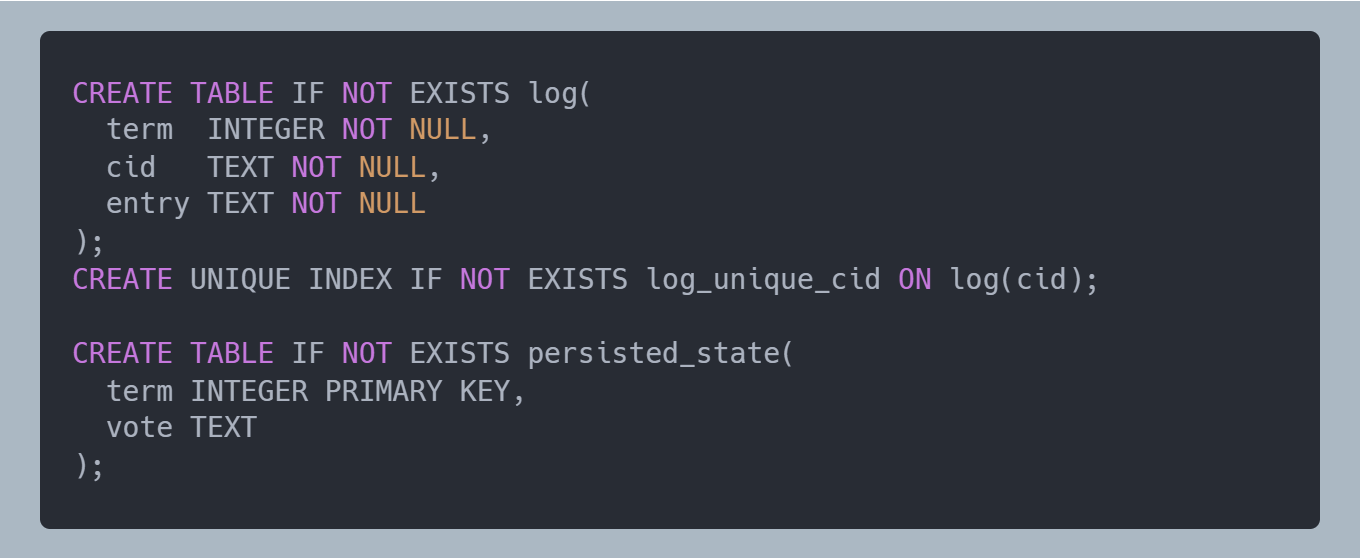
\includegraphics[width=400pt]{images/sqlite-schema.png}
  \caption{Schema used to implement Raft's persistence layer.}
  \label{fig:sqlite-schema}
\end{figure}

\subsection{REST API Specification for Server-To-Server Communication} \label{rpc-endpoints}

In addition to the client-facing endpoints described in the introduction of Section \ref{impl-overview}, there are two more defined for message-passing between servers.
%%begin novalidate
\begin{enumerate}
    \item \lstinline|PUT /raft/append_entries|: Is called by external servers to send an \lstinline|AppendEntries| request. An HTTP body containing the request encoded as JSON is expected. 
    \item \lstinline|PUT /raft/request_vote|: Is called by external servers to send a \lstinline|RequestVote| request. An HTTP body containing the request encoded as JSON is expected.
\end{enumerate}
%%end novalidate

\section{Testing Cluster Deployment} \label{testing-cluster-deployment}

The key-value store module is packaged into a Docker image using Sbt. The configuration for achieving this can be found in the \lstinline|build.sbt| file at the root of the project's source code.\\

Additionally, the key-value store comes with a configuration for deploying a cluster of servers in Docker containers, along with an Nginx reverse proxy, using Docker Compose. This setup is used for experimenting and testing the system, but is not adequate for a production setting. Its main flaw is the single Nginx instance, which is a single point of failure and potentially a bottleneck. These flaws are not relevant though, since this setup's only purpose is to verify the store's behavior and would not be used in a production deployment.\\

The Docker Compose configuration is shown in Figures \ref{fig:kvstore-docker-compose-A} and \ref{fig:kvstore-docker-compose-B}. Each part is described in detail, since it provides a complete and succinct overview of how a Raft cluster is typically structured.

\begin{figure}[ht]
  \centering
  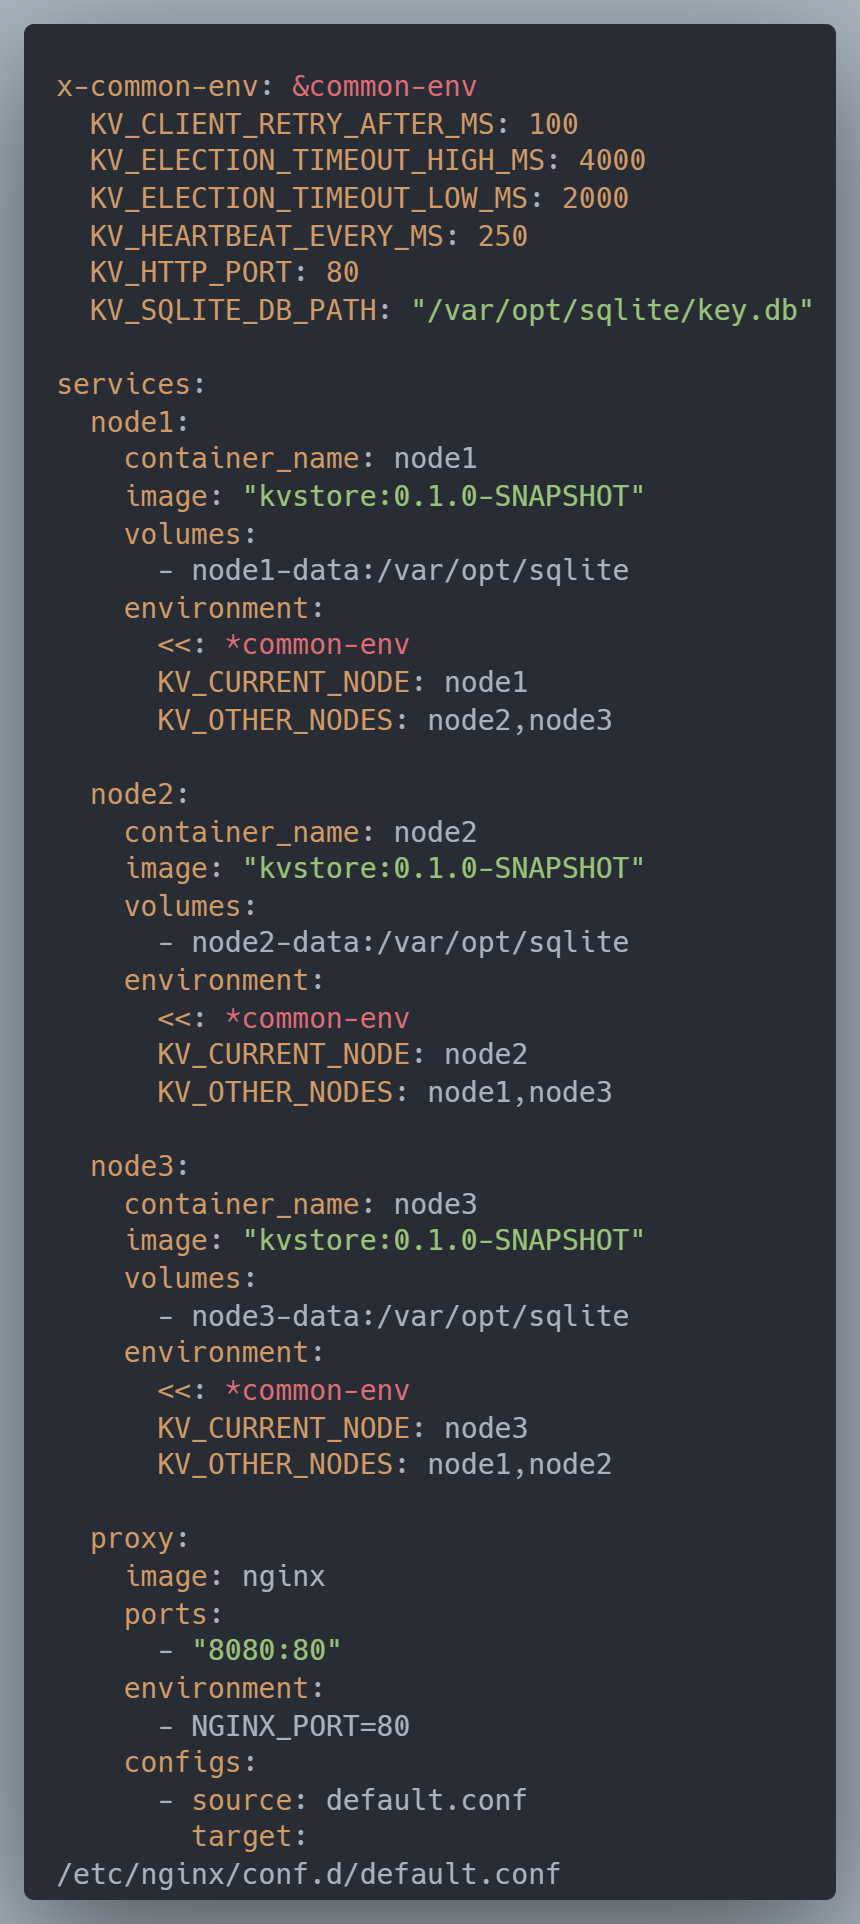
\includegraphics[width=265pt]{images/kvstore-docker-compose-A.png}
  \caption{First part of the Docker Compose configuration. It shows the configuration for deploying three key-value store servers, along with an Nginx proxy. The proxy configuration along with the definition of the required data volumes are shown in Figure \ref{fig:kvstore-docker-compose-B}.}
  \label{fig:kvstore-docker-compose-A}
\end{figure}

\begin{figure}[ht]
  \centering
  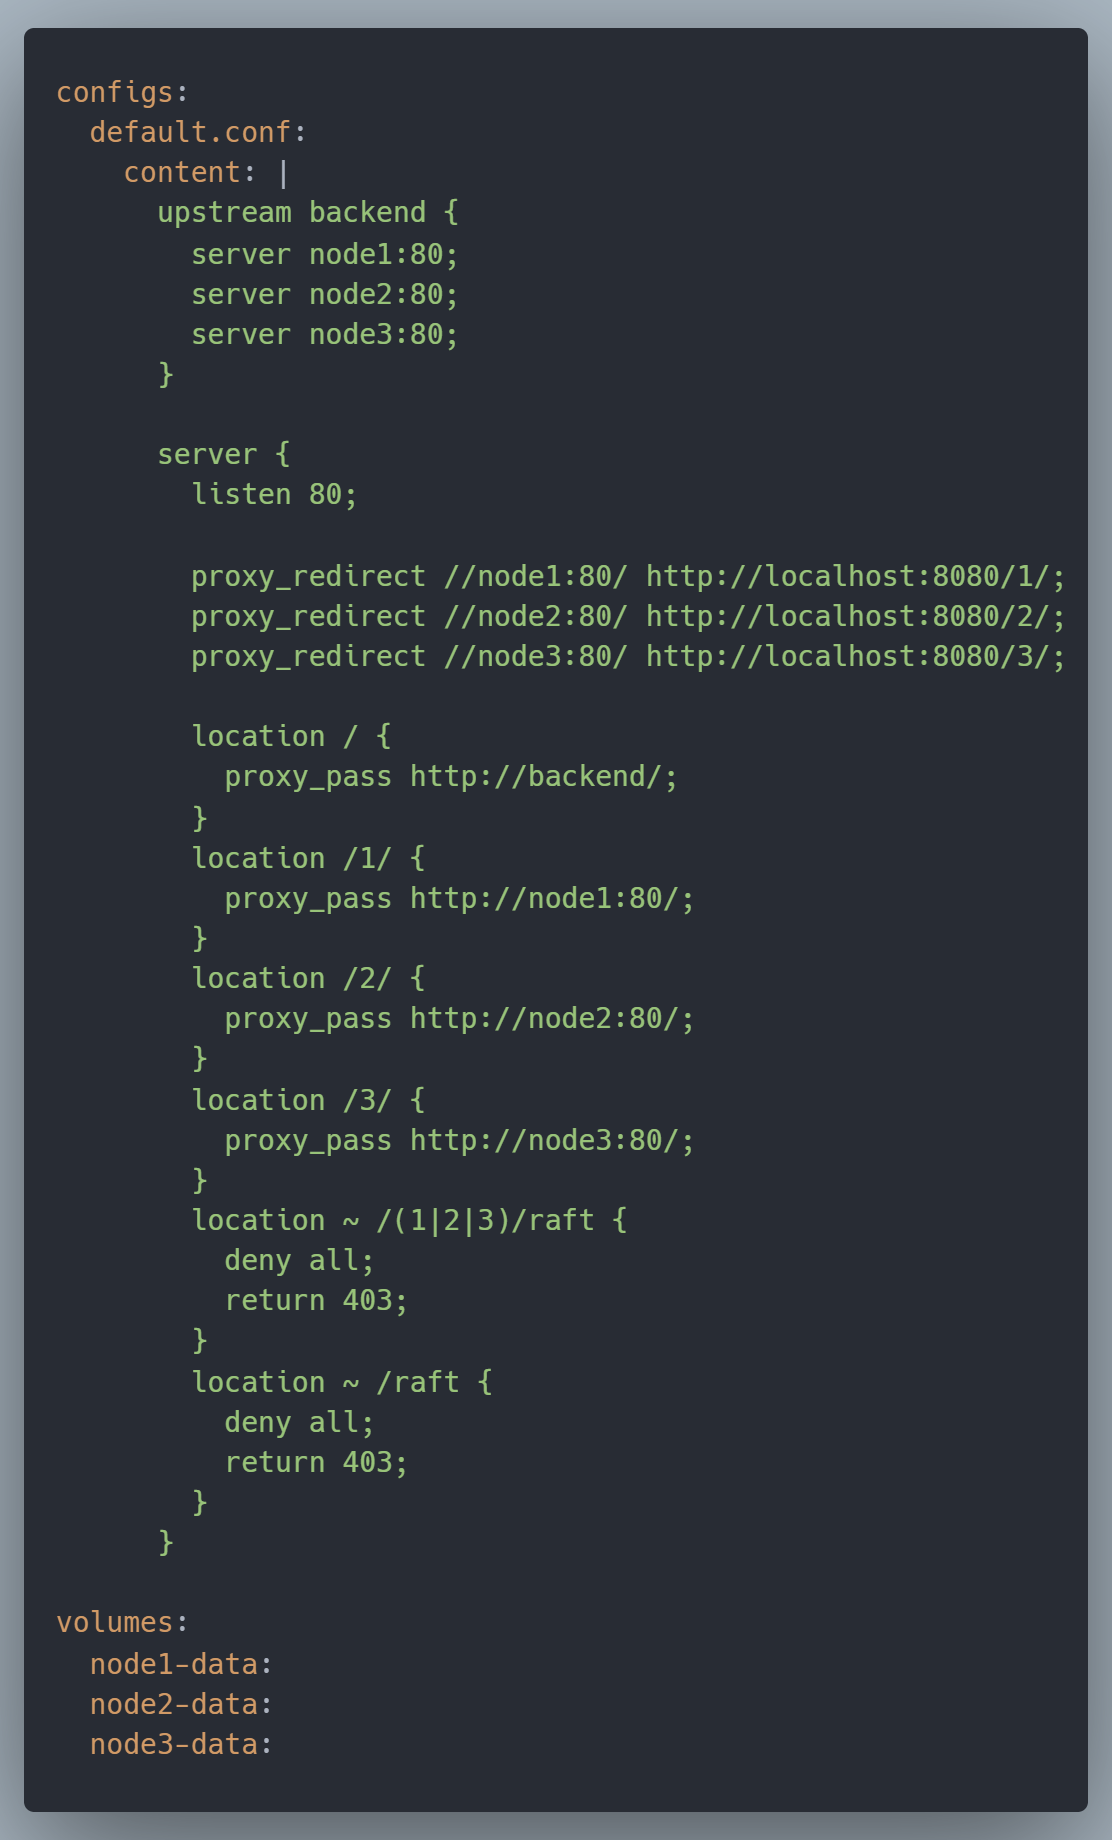
\includegraphics[width=350pt]{images/kvstore-docker-compose-B.png}
  \caption{Continuation of Figure \ref{fig:kvstore-docker-compose-A}, showing the configuration for the Nginx reverse proxy along with the definition of the required data volumes.}
  \label{fig:kvstore-docker-compose-B}
\end{figure}

\subsection{Key-Value Store Server Configuration}

As shown in Figure \ref{fig:kvstore-docker-compose-A}, three key-value store servers are deployed. All of them use identical values for some configuration parameters, which are placed in the \lstinline|x-common-env| object and injected into the environment sections of all servers:
\begin{itemize}
  \item \lstinline{KV_CLIENT_RETRY_AFTER_MS}: How long to wait between retries when a server-to-server communication fails. It is set to 100 milliseconds.
  \item \lstinline{KV_ELECTION_TIMEOUT_HIGH_MS}: The upper bound for the election timeout range. It is set to 4000 milliseconds, or 4 seconds.
  \item \lstinline{KV_ELECTION_TIMEOUT_LOW_MS}: The lower bound for the election timeout range. It is set to 2000 milliseconds, or 2 seconds.
  \item \lstinline{KV_HEARTBEAT_EVERY_MS}: The heartbeat interval. It is set to 250 milliseconds.
  \item \lstinline{KV_HTTP_PORT}: The port that the HTTP server listens to for all communications. It is set to the default HTTP port, 80.
  \item \lstinline{KV_SQLITE_DB_PATH}: The location in each container's file system that Sqlite places its database file. It is set to \lstinline{/var/opt/sqlite/key.db}.
\end{itemize}

Furthermore, all servers are configured with their own unique identifier, under \lstinline{KV_CURRENT_NODE}, and with the identifiers of the other servers, under \lstinline{KV_OTHER_NODES}. The identifiers match the container names of each server, which ultimately map to their hostnames within the cluster, as they are part of the same Docker network. As a result, knowing a server's identifier is enough to send an HTTP request to it from within the Docker network simply by using the identifier as the target hostname.

\subsection{Proxy Configuration and Redirects}

Although the server containers would be adequate for implementing the distributed key-value store, there are several problems and inconveniences that need to be addressed:
\begin{enumerate}
    \item The servers belong in a single docker network without exposing any ports, meaning that they are not reachable from the outside.
    \item If the servers were to expose their ports directly to the outside, clients would need to implement some sort of discovery procedure for learning their locations. This leaks implementation details and forces the cluster to remain as static as possible to not force clients to go through additional discovery procedures.
    \item Each server exposes its entire set of endpoints under the same port, including the ones that should not be accessed by clients. This allows clients to perform arbitrary actions within the Raft cluster, since there is no authorization mechanism in place.
\end{enumerate}

Nginx is used as a reverse proxy to address all these problems, and its configuration is shown in Figure \ref{fig:kvstore-docker-compose-B}. \\ 

To address the first two problems, the Nginx container exposes a port, which clients can use for interacting with the key-value store. A client can address the cluster as a whole, allowing Nginx to route the request to one of the servers. This is achieved by grouping all the servers with the \lstinline{backend} upstream, which is reachable via the \lstinline{/} path. The discovery process is simplified, since a client can address the cluster as a whole, and it will be redirected to the proper recipient for its request. Additionally, after a client learns about a specific server, it can address it by prefixing an endpoint with the server's number. \\

The Nginx configuration also disallows any access to endpoints prefixed with \lstinline{raft}. These must only be called by other servers, as they are used for appending entries and requesting votes.\\

Note that this configuration assumes a static setup, where servers are not added or removed dynamically. The shape of the cluster can only change through an interruption of service, where all the servers and the proxy are shut down, reconfigured, and then redeployed.

\subsection{Data Volumes}

Each server is configured with a unique Docker volume, used to persist the Sqlite database in the file system. The volumes' configuration is shown in Figure \ref{fig:kvstore-docker-compose-B}, while their usage is shown in Figure \ref{fig:kvstore-docker-compose-A}. Having these volumes means that containers can be freely shut down and restarted without data loss.

\section{Linearizable Semantics} \label{linearizable-semantics}

As mentioned several times before, Raft makes several design choices to support linearizable semantics. This is explained in detail in Chapter 6 of the original Raft paper \cite{raft}. The key-value store implementation also supports linearizable semantics, but in a simplified fashion.

\subsection{Requirements of Linearizable Semantics}

Linearizable semantics are important for making a distributed system easy to reason about. The authors of the Raft paper describe them as follows: "In linearizability, each operation appears to execute instantaneously, exactly once, at some
point between its invocation and its response."\cite{raft}.\\

To implement them, there are two requirements that the Raft implementation must fulfill \cite{raft}: 
\begin{enumerate}
    \item Any operation, read or write, must be executed based on an up-to-date view of the system's state and return a response only once committed.
    \item Operations must get executed exactly once.
\end{enumerate}

\subsection{Implementation of Linearizable Semantics in the Key-Value Store}

To address the first requirement, all commands are routed to the leader, which is the single authority on the current state of the system. Before returning a response, the leader appends the command to its log and attempts to commit it by replicating it to the rest of the cluster. Importantly, this also encompasses commands which simply read from the state; the Raft implementation appends them in the log like any other command before replying. This ensures that the leader is still the authority on the current state when responding, as it successfully manages to commit an entry.\\

The second requirement is fulfilled by expecting clients to include a unique identifier along with their commands. If a command is somehow received twice by the system, due to the client retrying, a duplication caused by the network, or another reason, it is identified as a duplicate using its id and it is rejected. The command ids are also stored in the log, so they are completely durable. Note that this implementation is far simpler than how it is described in the original Raft paper, which also stores the response and returns it instead of rejecting the duplicate command, using a session mechanism. Although this would be a more complete solution, it adds a lot of implementation overhead and it was deemed not worthwhile for the key-value store.
